% ---------------------------------------------------------------------------------------
\chapter{Coeficientes para la
comparaci\'on entre dos
imagenes}\label{chap3}

La creciente dimensionalidad de los conjuntos de datos utulizados comunmente ha llevado a la popularidad el concepto de la ciencia generadora de hip\'otesis, en la cual los conjuntos de datos se utilizan para ayudar a los investigadores a formular nuevas hip\'otesis en lugar de probar las existentes. En este enfoque, se utilizan medidas de dependencia, que son estad\'isticas empleadas para evaluar pares de variables candidatas. Estos avances en el campo de analisis de datos nos han entregado muchas herramientas, tanto para la comparaci\'on de datos en si mismos, junto con formas de evaluar estas medidas en si mismas. 

Una manera de medir la utilidad de una medida de dependencia $\hat\varphi$ es la potencia contra la independencia, es decir, la capacidad de prueba de independencia basada en $\hat\varphi$ para detectar varios tipos de relaciones no triviales. Este es un objetivo importante para conjuntos de datos que tienen muy pocas relaciones no triviales, o solo relaciones muy d\'ebiles que son dif\'iciles de detectar. Sin embargo, a menudo el n\'umero de relaciones declaradas estad\'isticamente significativas por una medida de dependencia supera con creces el n\'umero de relaciones que luego se pueden explorar m\'as a fondo.

Para abordar este problema, se introdujo un segundo m\'etodo de evaluaci\'on de una medida de dependencia llamado equitabilidad \cite{Reshef2011}. Las estad\'isticas equitativas asignan puntuaciones similares a relaciones igualmente fuertes, independientemente de su tipo. El objetivo es definir medidas de dependencia que logren una buena equitabilidad con respecto a medidas relevantes de la fuerza de la relaci\'on. 
B
La idea de equitabilidad ha motivado el desarrollo de varias medidas de dependencia, con diferentes formalizaciones y enfoques en aspectos espec\'ificos de la fuerza de la relaci\'on. El desaf\'io radica en definir medidas de dependencia que logren una buena equitabilidad con respecto a medidas importantes de la fuerza de la relaci\'on, como se ve en el art\'iculo complementario de Reshef et al. Esta l\'inea de investigaci\'on tiene como objetivo proporcionar un enfoque m\'as poderoso y equitativo para medir la dependencia, lo que permite una identificaci\'on y priorizaci\'on m\'as precisas de las relaciones en conjuntos de datos complejos.

Con esto en mente, en esta secci\'on estudiaremos el coeficiente de informaci\'on m\'axima (MIC), Correlaci\'on local, y la correlaci\'on de Pearson; los cuales son los coeficientes m\'as utilizados para la comparaci\'on entre dos imagenes. Notemos que que ya fue mostrado por Reshef et al (2011) que el coeficiente de informaci\'on m\'axima (MIC) es equitativo, estudiaremos la equitatividad de los otros dos coeficientes m\'as adelante.

\section[]{\textit{Maximal Information Coeficient}}
%Reshef.SOM.v2.pdf

\subsection{Sobre el coeficiente}

	El coeficiente de informaci\'on m\'axima (Maximal Information Coefficient o MIC) es una medida estad\'istica propuesta por Reshef et al. en su paper "Detecting Novel Associations in Large Data Sets" \cite{Reshef2011}. Este coeficiente mide la correlaci\'on entre dos variables en un conjunto de datos y se basa en la idea de que una relaci\'on fuerte entre dos variables deber\'ia ser capaz de predecir una variable a partir de la otra de manera precisa.

	En su paper, Reshef et al. presentan un enfoque innovador para detectar asociaciones nobles en grandes conjuntos de datos, en lugar de buscar correlaciones fuertes entre dos variables, el coeficiente MIC permite detectar relaciones d\'ebiles pero a\'un importantes que pueden no ser evidentes al simplemente mirar los datos. Esto es posible gracias a que el coeficiente MIC es capaz de capturar no solo la fuerza de la correlaci\'on entre dos variables, sino tambi\'en su precisi\'on.

	Para calcular el coeficiente, se parte de la idea de que la informaci\'on mutua entre dos variables es una medida de la precisi\'on con la que se puede predecir una variable a partir de la otra. Por lo tanto, el coeficiente se calcula como la informaci\'on mutua m\'axima posible entre dos variables, dado un conjunto de datos. Esto se hace a trav\'es de un procedimiento iterativo en el que se prueban diferentes particiones de los datos en conjuntos de entrenamiento y prueba, y se selecciona aquella que maximiza la informaci\'on mutua.

	El la siguiente secci\'on estudiaremos las definiciones que nos entrega cada coeficiente.
 
\subsection{Definiciones}

	Como mencionamos en la parte anterior, debemos primero encontrar la informaci\'on mutua entre las variables, para esto definamos:

	\begin{defn}[Informaci\'on mutua]
		Para dos variables aleatorias conjuntas $X$ e $Y$, se define la informaci\'on mutua como:
		$$
		\mathrm{I}(X ; Y)=\int_{\mathcal{Y}} \int_{\mathcal{X}} P_{(X, Y)}(x, y) \log \left(\frac{P_{(X, Y)}(x, y)}{P_{X}(x) P_{Y}(y)}\right)dxdy
		$$
		Donde $P_{(X, Y)}$ es la funci\'on de densidad de probabilidad conjunta y $P_{X}$, $P_{Y}$, las distribuciones marginales de $X$ e $Y$ respectivamente. 
	\end{defn}

	Luego, sea $D$ un conjunto finito de pares ordenados, podemos particionar los valores de la primera coordenada en $x$ contenedores, y los valores de la segunda en $y$ de estos. Dado una malla $G$, sea $D|_G$ la distribuci\'on inducida pokr los puntos de $D$ en las celdas de $G$, i.e., la distribuci\'on en las celdas de $G$ obtenida al dejar que la funci\'on de densidad de probabilidad en cada celda sea la fracci\'on de puntos de $D$ que caen en esa celda. Veamos un ejemplo
	\begin{figure}[H]\label{malla_G}
		\centering
		\includegraphics*[scale = 0.4]{D_G_example1.png}
		\caption{Malla G de 4x3 sobre el conjunto de pares ordenados D, figura no final}
	\end{figure}

	Para la figura \ref{malla_G}, la funci\'on de densidad quedar\'ia de la forma:
	\[
		f_{D|_G}(i,j) = \left\{\begin{array}{lr}
			\frac{2}{10} & \text{si } (i,j) \in \{ (1,1), (2,2), (4,2)\} \\
			\frac{1}{10}, & \text{si }(i,j) \in \{ (3,2)\}  \\
			\frac{3}{10}, & \text{si }(i,j) \in \{ (4,1)\}  \\
			0, & \text{Otro caso.}
			\end{array}\right.
	\]



	Notemos que para un $D$ fijo, aunque fijemos el grosor de la malla, la distrion de esta puede variar dependiendo de donde hagamos los cortes, por ejemplo:

	\begin{figure}[H] \label{malla_G_2}
		\centering
		\includegraphics*[scale = 0.4]{D_G_example2.png}
		\caption{Otra malla G de 4x3 sobre el conjunto de pares ordenados D, figura no final}
	\end{figure}

	Aqu\'i podemo ver que la funci\'on de densidad que nos entrega est\'a malla es distinta a la definida para la figura \ref{malla_G_2}. Este es un hecho que explotamos en la siguiente definici\'on: 

	\begin{defn}
		Para un conjunto finito $D\in\R^2$ y enteros positivos $i,j$, definimos:
		$$
		I^*(D,i,j)=\max I(D|_G)
		$$
		donde el m\'aximo es sobre todas las mallas $G$ con $i$ columnas y $j$ filas, con $I(D|_G)$ denot la informaci\'on mutua de $D|_G$.
	\end{defn}

	Ya teniendo este valor procedemos a definir la matriz caracteristica del conjunto $D$.

	\begin{defn}
		La matriz caracteristica $M(D)$ de un conjunto bivariado $D$ es una matriz infinita con entradas:
		$$
		M(D)_{x, y}=\frac{I^{*}(D, x, y)}{\log \min \{x, y\}}
		$$
	\end{defn}
	\begin{defn}
		El coeficiente de informaci\'on m\'axima o \textit{MIC} de un conjunto bivariado $D$ de tama\~no $n$ y una malla de tama\~no menos a $B(n)$ esta dado por:
		$$
		\operatorname{MIC}(D)=\max _{x y<B(n)}\left\{M(D)_{x, y}\right\}
		$$
		donde $\omega(1)<B(n) \leq O\left(n^{1-\varepsilon}\right)$ para alg\'un $0<\varepsilon<1$ 
	\end{defn}
	\begin{rem}
		A menos que se especifique de otra forma, al momento de trabajar con esta medida usaremos $B(n)=n^{0.6}$, que es la funci\'on que ocupan en el paper citado al principio del la secci\'on
	\end{rem}

	\subsection{Formas pr\'acticas de calcular el MIC, el $MIC_*$, $TIC_e$ y $MIC_e$}

	En el art\'iculo "Measuring Dependence Powerfully and Equitably" de Reshef et al., los autores presentan y caracterizan te\'oricamente dos nuevas medidas de dependencia: $MIC_*$ y $MIC_e$. $MIC_*$ es una medida de dependencia poblacional, y el art\' iculo presenta tres formas de ver esta cantidad. Los autores demuestran que $MIC_*$ es el valor poblacional del coeficiente de informaci\'on m\'axima (MIC), una suavizaci\'on m\'inima de la informaci\'on mutua y el supremo de una secuencia infinita. Estas caracterizaciones simplifican el c\'alculo y fortalecen los resultados te\'oricos.

	Adem\'as, los autores desarrollan algoritmos eficientes para aproximar $MIC_*$ en la pr\'actica y estimarlo de manera consistente a partir de una muestra finita. Introducen $MIC_e$, un estimador consistente de $MIC_*$, que es computable de manera eficiente y m\'as r\'apido en la pr\'actica que el algoritmo heur\'istico para calcular MIC. A trav\'es de simulaciones, demuestran que $MIC_e$ tiene mejores propiedades de sesgo/varianza y supera a los m\'etodos existentes en t\'erminos de equitabilidad con respecto a R2 en un amplio conjunto de relaciones funcionales ruidosas.

	\subsection[short]{Definiciones y propiedades de $MIC_*$}

	En esta secci\'on, abordaremos las definiciones esenciales para el c\'alculo del $MIC_e$. El coeficiente m\'aximo de informaci\'on poblacional puede expresarse de diversas maneras equivalentes, como veremos m\'as adelante. Sin embargo, comenzaremos con la definici\'on m\'as sencilla.

	\begin{defn}
		Sea $(X,Y)$ una pareja de variables aleatorias conjuntamente distribuidas. El coeficiente de informaci\'on m\'axima poblacional ($MIC_*$) de $(X,Y)$ se define como:
		$$
		M I C_*(X, Y)=\sup _G \frac{I\left(\left.(X, Y)\right|_G\right)}{\log \|G\|}
		$$
		
		donde $||G||$ denota el m\'inimo entre el n\'umero de filas y el n\'umero de columnas de G.
	\end{defn}
	
	Ya que $I(X,Y) = sup_G I((X,Y)|G)$ (consultar, por ejemplo, el Cap\'itulo 8 de Cover y Thomas, 2006), esto puede interpretarse como una versi\'on regularizada de la informaci\'on mutua que sanciona las rejillas complejas y garantiza que el resultado est\'e dentro del rango entre cero y uno.
	
	Previo a continuar, introducimos una definici\'on equivalente y sencilla de $MIC_*$ que resulta \'util para los resultados en esta secci\'on. Esta definici\'on considera a $MIC_*$ como el supremo de una matriz denominada matriz caracter\'istica poblacional, que se define a continuaci\'on.
	
	\begin{defn}
		Sea $(X,Y)$ una pareja de variables aleatorias conjuntamente distribuidas. Sea
		$$
		I^*((X, Y), k, \ell)=\max _{G \in G(k, \ell)} I\left(\left.(X, Y)\right|_G\right)
		$$
		La matriz caracter\'istica poblacional de (X,Y), denotada por M(X,Y), se define como
		$$
		M(X, Y)_{k, \ell}=\frac{I^*((X, Y), k, \ell)}{\log \min \{k, \ell\}}
		$$
	\end{defn}
	
	para $k$, $l > 1$.
	
	Es f\'acil ver lo siguiente:

	
	Proposici\'on 3: Sea $(X,Y)$ una pareja de variables aleatorias conjuntamente distribuidas. Tenemos
	
	$$MIC*(X,Y) = sup M(X,Y)$$
	
	donde $M(X,Y)$ es la matriz caracter\'istica poblacional de $(X,Y)$.
	
	La matriz caracter\'istica poblacional recibe este nombre porque, al igual que el MIC*, el supremo de esta matriz, captura una noci\'on de la intensidad de la relaci\'on, y otras propiedades de esta matriz se relacionan con diferentes caracter\'isticas de las relaciones. Por ejemplo, m\'as adelante en este documento presentamos una propiedad adicional de la matriz caracter\'istica, el coeficiente de informaci\'on total, que es \'util para comprobar la presencia o ausencia de una relaci\'on en lugar de cuantificar la intensidad de la relaci\'on.

	\section[short]{El $MIC_*$ es el valor poblacional del $MIC$}

	Con el $MIC_*$ definido, presentamos nuestra primera caracterizaci\'on alternativa de este, como el l\'imite de muestra grande del estad\'istico MIC introducido en Reshef et al. \cite{Reshef2011}. Recordemos la Definiciones del MIC y la matriz caracter\'istica de muestra. Notemos que para evistar confuci\'on denotaremos como $MIC$ al estad\'istico MIC y como $MIC_*$ al coeficiente de informaci\'on m\'axima poblacional.

	\begin{defn}
		(Reshef et al., 2011)  Sea $D \subset \mathbb{R}^2$ un conjunto de pares ordenados. La matriz caracter\'istica de muestra $\widehat{M}(D)$ de $D$ se define por
		$$
		\widehat{M}(D)_{k, \ell}=\frac{I^*(D, k, \ell)}{\log \min \{k, \ell\}} .
		$$
	\end{defn}

	\begin{defn}
		(Reshef et al., 2011) Sea $D \subset \mathbb{R}^2$ un conjunto de $n$ pares ordenados, y sea $B$ : $\mathbb{Z}^{+} \rightarrow \mathbb{Z}^{+}$. Definimos
		$$
		M I C(D)=\max _{k \ell \leq B(n)} \widehat{M}(D)_{k, \ell}
		$$
	\end{defn}

	Donde la funci\'on B(n) es especificada por el usuario. En el paper se sugiri\'o que B(n) se elija como $n^\alpha$ para alguna constante $\alpha$ en el rango de 0.5 a 0.8. (Los estad\'isticos que presentaremos m\'as adelante tendr\'an un par\'ametro an\'alogo; v\'ease la Secci\'on 4.4.1.)

	El siguiente resultado, demostrado en el paper de Reshef 2016, sobre la convergencia de funciones de la matriz caracter\'istica de muestra a sus contrapartes poblacionales, una consecuencia de lo cual es la convergencia de MIC a $MIC_*$. (En la declaraci\'on del teorema a continuaci\'on, recordemos que $m_\infty$ es el espacio de matrices infinitas equipadas con la norma supremo, y dada una matriz A, la proyecci\'on ri anula todas las entradas $A_{k, \ell}$ para las cuales $k\ell > i.$)

	\begin{thm}
		Sea $f: m^{\infty} \rightarrow \mathbb{R}$ uniformemente continua, y suponga que $f \circ r_i \rightarrow f$ puntualmente. Entonces, para cada variable aleatoria $(X, Y)$, tenemos
		$$
		\left(f \circ r_{B(n)}\right)\left(\widehat{M}\left(D_n\right)\right) \rightarrow f(M(X, Y))
		$$
		en probabilidad donde $D_n$ es una muestra de tama\~no $n$ de la distribuci\'on de $(X, Y)$, siempre que $\omega(1)<B(n) \leq O\left(n^{1-\varepsilon}\right)$ para alg\'un $\varepsilon>0$.
	\end{thm}

	Dado que el supremo de una matriz es una funci\'on uniformemente continua en $m_\infty$ y se puede realizar como el l\'imite de m\'aximos de segmentos cada vez m\'as grandes de la matriz, este teorema genera nuestra afirmaci\'on sobre $MIC_*$ como corolario.

	Corolario 7: $MIC$ es un estimador consistente de $MIC_*$ siempre que $\omega(1) < B(n) \leq O(n^{1-\epsilon})$ para alg\'un $\epsilon > 0$.

	Ya con esto podemos trabajar, bajo ciertas condiciones, con el $MIC_*$ como reemplazo del $MIC$. Pero, ¿Cu\'al es la ventaja de trabajar con este nuevo estimador? En pocas palabras, es m\'as f\'acil de estimar, y esto lo veremos en la en una secci\'on m\'as adelante. Antes de esto debemos revisar una caracterizaci\'on del $MIC_*$ que nos permitir\'a contruir un estimador de este.

	\subsection[short]{El $MIC_*$ es el supremo de la matriz caracter\'istica de muestra}

	Ahora mostramos la una vista alternativa de $MIC_*$: que puede definirse de manera equivalente como el supremo sobre un l\'imite de la matriz caracter\'istica en lugar de como un supremo sobre todas las entradas de la matriz. Esta caracterizaci\'on de $MIC_*$ servir\'a como base tanto para nuestro enfoque de aproximaci\'on de $MIC_*(X, Y)$ como para el nuevo estimador de $MIC_*$ que presentamos m\'as adelante en este art\'iculo.

	Comenzamos definiendo lo que entendemos por l\'imite de la matriz caracter\'istica. Nuestra definici\'on se basa en la siguiente observaci\'on.
	\begin{prop}
		Sea $M$ una matriz caracter\'istica poblacional. Entonces, para $\ell \geq k, M_{k, \ell} \leq M_{k, \ell+1}$
	\end{prop}
	\begin{proof}
		Sea $(X, Y)$ la variable aleatoria en cuesti\'on. Dado que siempre podemos dejar una fila/columna vac\'ia, sabemos que $I^*((X, Y), k, \ell) \leq I^*((X, Y), k, \ell+1)$. Y dado que $\ell, \ell+1 \geq k$, sabemos que $M_{k, \ell}=I^*((X, Y), k, \ell) / \log k \leq I^*((X, Y), k, \ell+1) / \log k=M_{k, \ell+1}$.
	\end{proof}

	Dado que las entradas de la matriz caracter\'istica est\'an acotadas, el teorema de convergencia mon\'otona nos da el siguiente corolario. En el corolario y en adelante, dejamos $M_{k, \uparrow}=\lim _{\ell \rightarrow \infty} M_{k, \ell}$ y definimos $M_{\uparrow, \ell}$ de manera similar.
	\begin{cor}
		Sea $M$ una matriz caracter\'istica poblacional. Entonces, $M_{k, \uparrow}$ existe, es finito e igual a $\sup _{\ell \geq k} M_{k, \ell}$. Lo mismo es v\'alido para $M_{\uparrow, \ell}$.
	\end{cor}

	El corolario anterior nos permite definir el l\'imite de la matriz caracter\'istica.

	\begin{defn}
		Sea $M$ una matriz caracter\'istica poblacional. El l\'imite de $M$ es el conjunto
		$$
		\partial M=\left\{M_{k, \uparrow}: 1<k<\infty\right\} \bigcup\left\{M_{\uparrow, \ell}: 1<\ell<\infty\right\}
		$$
	\end{defn}
	
	El teorema siguiente da una relaci\'on entre el l\'imite de la matriz caracter\'istica y $\mathrm{MIC}_*$.
	\begin{thm}
	Sea $(X, Y)$ una variable aleatoria. Tenemos
	$$
	M I C_*(X, Y)=\sup \partial M(X, Y)
	$$
	donde $M(X, Y)$ es la matriz caracter\'istica poblacional de $(X, Y)$.
	\end{thm}
	\begin{proof}
		El siguiente argumento muestra que cada entrada de $M$ es, como m\'aximo, $\sup \partial M$: fije un par $(k, \ell)$ y observe que, o bien $k \leq \ell$, en cuyo caso $M_{k, \ell} \leq M_{k, \uparrow}$, o bien $\ell \leq k$, en cuyo caso $M_{k, \ell} \leq M_{\uparrow, \ell}$. 
		
		Por lo tanto, 
		
		$\mathrm{MIC}_* \leq \sup \left\{M_{\uparrow, \ell}\right\} \cup\left\{M_{k, \uparrow}\right\}=\sup \partial M$
	\end{proof}
	
	Por otro lado, el Corolario muestra que cada elemento de $\partial M$ es un supremo sobre algunos elementos de $M$. Por lo tanto, sup $\partial M$, al ser un supremo sobre supremos de elementos de $M$, no puede exceder $\sup M=\mathrm{MIC}_*$.


	\section{Estimando el $MIC_*$ con $MIC_e$}

	Como hemos revisado, $MIC_*$ es el valor poblacional del estad\'istico MIC introducido en Reshef et al. (2011). Sin embargo, aunque es consistente, el estad\'istico MIC no se conoce por ser eficientemente computable y en Reshef et al. (2011) se calcul\'o en su lugar un algoritmo heur\'istico de aproximaci\'on llamado Approx-MIC. En esta secci\'on, revisaremos un estimador de $MIC_*$ que es tanto consistente como eficientemente computable. El nuevo estimador, llamado $MIC_e$, tiene una mejor complejidad de tiempo de ejecuci\'on incluso que el algoritmo heur\'istico Approx-MIC y es \'ordenes de magnitud m\'as r\'apido en la pr\'actica.

	El estimador $MIC_e$ se basa en una de las caracterizaciones alternativas de $MIC_*$ probadas en la secci\'on anterior. Espec\'ificamente, si $MIC_*$ puede considerarse como el supremo del l\'imite de la matriz caracter\'istica en lugar de la matriz completa, entonces solo el l\'imite de la matriz debe estimarse con precisi\'on para estimar $MIC_*$. Esto tiene la ventaja de que, mientras que calcular entradas individuales de la matriz caracter\'istica de muestra implica encontrar rejillas \'optimas (bidimensionales), estimar las entradas del l\'imite nos requiere solo encontrar particiones \'optimas (unidimensionales). Si bien el primer problema es computacionalmente dif\'icil, el segundo puede resolverse utilizando el algoritmo de programaci\'on din\'amica de Reshef et al. (2011).

	En paper publicado Reshef (2016), esta idea es formalizada a travez de un objeto llamado la matriz equicaracter\'istica, la cual es denominadad $[M]$. La diferencia entre $[M]$ y la matriz caracter\'istica $M$ es la siguiente: mientras que la entrada $k, \ell$-th de $M$ se calcula a partir de la informaci\'on mutua m\'axima alcanzable utilizando cualquier cuadr\'icula de $k$-por- $\ell$, la entrada $k, \ell$-th de $[M]$ se calcula a partir de la informaci\'on mutua m\'axima alcanzable utilizando cualquier cuadr\'icula de $k$-por- $\ell$ que equiparticiona la dimensi\'on con m\'as filas/ 	columnas. \ref{fig:matriz_equicaracteristica} (Ver Figura 1.) A pesar de esta diferencia, a medida que la equipartici\'on en cuesti\'on se vuelve m\'as y m\'as fina, se vuelve indistinguible de una partici\'on \'optima del mismo tama\~no. Esta intuici\'on se puede formalizar para mostrar que el l\'imite de $[M]$ es igual al l\'imite de $M$, y por lo tanto que $\sup [M]=\sup M=\mathrm{MIC}*$. Entonces, se deducir\'a que estimar $[M]$ y tomar el supremo, como lo hicimos con $M$ en el caso de MIC, proporciona una estimaci\'on consistente de $\mathrm{MIC}*$.

	\section{La matriz equicaracter\'istica} 

	Ahora definimos la matriz equicaracter\'istica y mostramos que su supremo es efectivamente $MIC^*$. Para hacerlo, primero definimos una versi\'on de $I^*$ que equiparticiona la dimensi\'on con m\'as filas/columnas. Observe que en la definici\'on, los corchetes se utilizan para indicar la presencia de una equipartici\'on.

	\begin{figure} \label{fig:matriz_equicaracteristica}
		\centering
		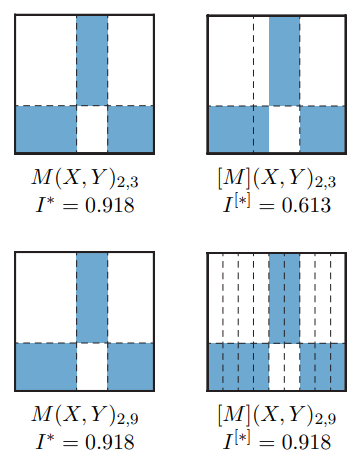
\includegraphics[scale=0.6]{figuras/figure_1_reshef_2016.png}
		\caption{Ejemplo de matriz equicaracteristica}
	\end{figure}
	
	{\textit{resumir la secci\'on 4 de Reshef 2016}}


	\subsection[]{Ejemplos}

	Ya con la funci\'on bien definida, veamos unos ejemplos del coeficiente, primero para algunos datos, y luego entre im\'agenes. Comenzemos por algunos ejemplos usando 

	el formato de esta secci\'on es temporal

	\begin{figure}[H]
		\centering
		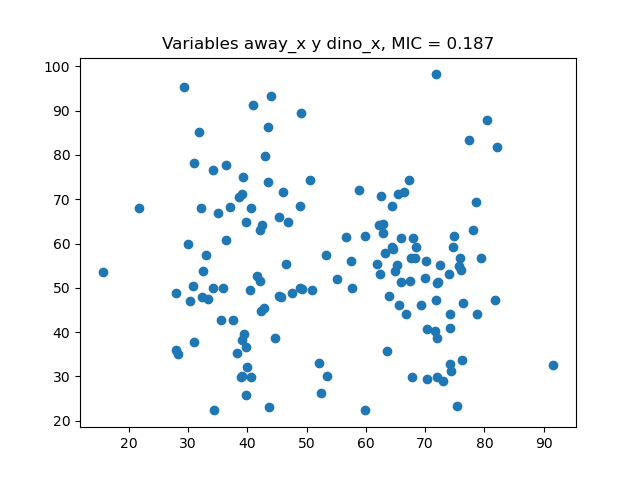
\includegraphics[scale=0.6]{away_x_dino_x_.png}
		\caption{ MIC = 0.187}
		\end{figure}
		
		\begin{figure}[H]
		\centering
		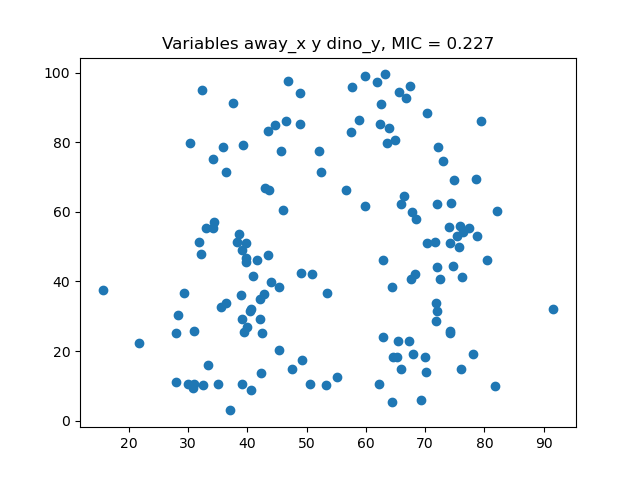
\includegraphics[scale=0.6]{away_x_dino_y_.png}
		\caption{ MIC = 0.227}
		\end{figure}
		
		\begin{figure}[H]
		\centering
		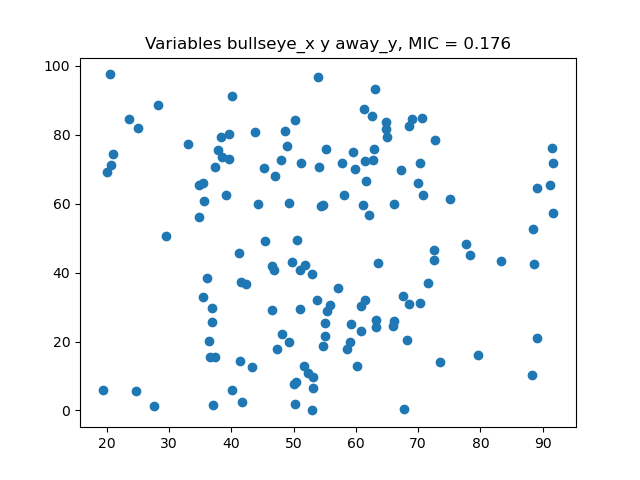
\includegraphics[scale=0.6]{bullseye_x_away_y_.png}
		\caption{ MIC = 0.176}
		\end{figure}
		
		\begin{figure}[H]
		\centering
		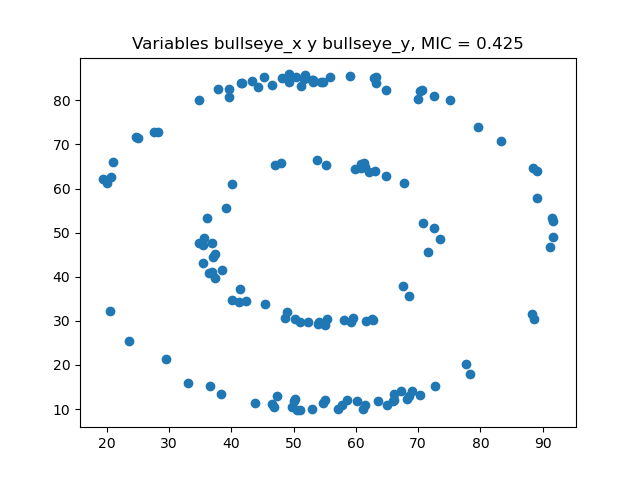
\includegraphics[scale=0.6]{bullseye_x_bullseye_y_.png}
		\caption{ MIC = 0.425}
		\end{figure}
		
		\begin{figure}[H]
		\centering
		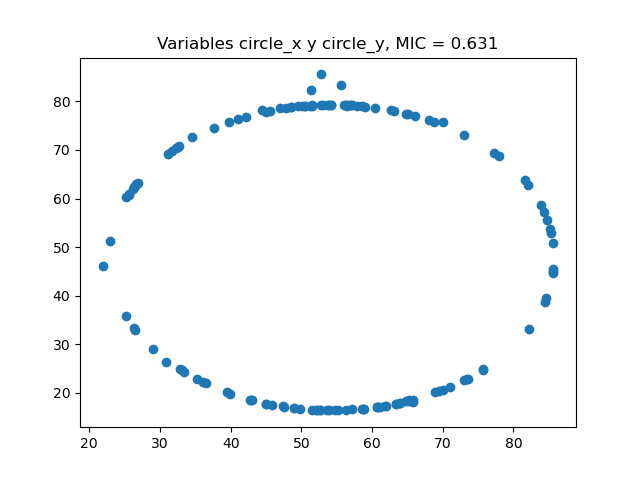
\includegraphics[scale=0.6]{circle_x_circle_y_.png}
		\caption{ MIC = 0.631}
		\end{figure}
		
		\begin{figure}[H]
		\centering
		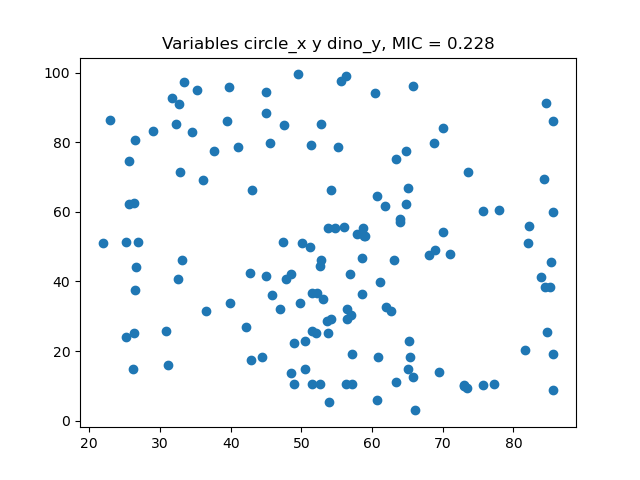
\includegraphics[scale=0.6]{circle_x_dino_y_.png}
		\caption{ MIC = 0.228}
		\end{figure}
		
		\begin{figure}[H]
		\centering
		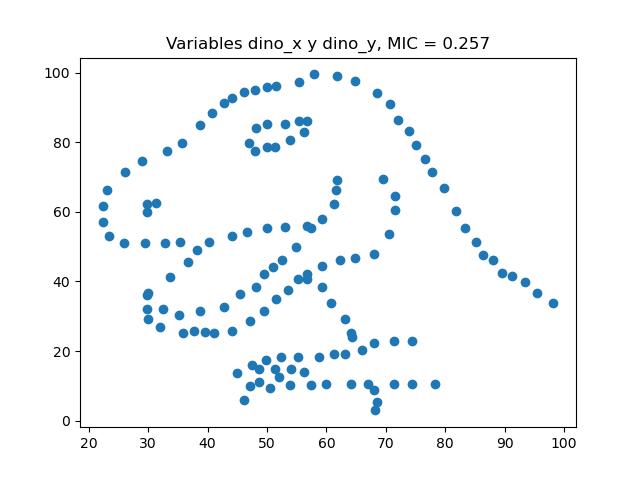
\includegraphics[scale=0.6]{dino_x_dino_y_.png}
		\caption{ MIC = 0.257}
		\end{figure}
		
		\begin{figure}[H]
		\centering
		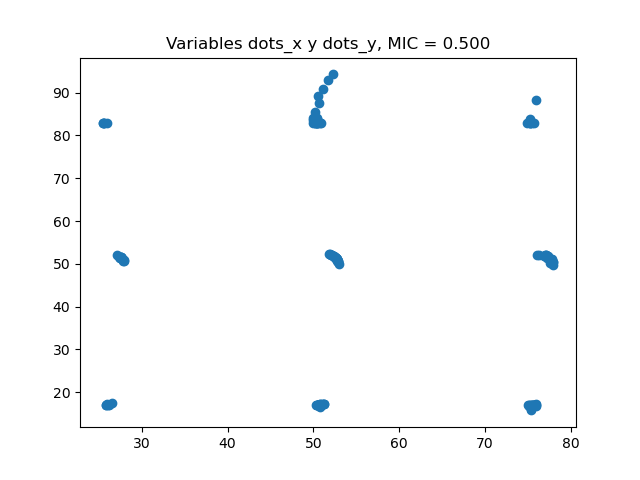
\includegraphics[scale=0.6]{dots_x_dots_y_.png}
		\caption{ MIC = 0.500}
		\end{figure}
		
		\begin{figure}[H]
		\centering
		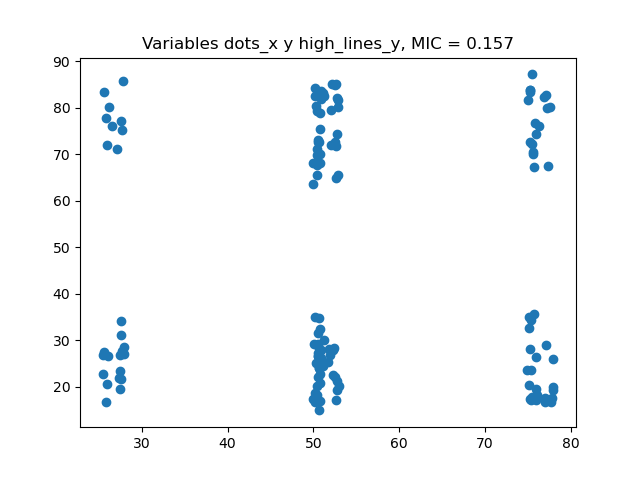
\includegraphics[scale=0.6]{dots_x_high_lines_y_.png}
		\caption{ MIC = 0.157}
		\end{figure}
		
		\begin{figure}[H]
		\centering
		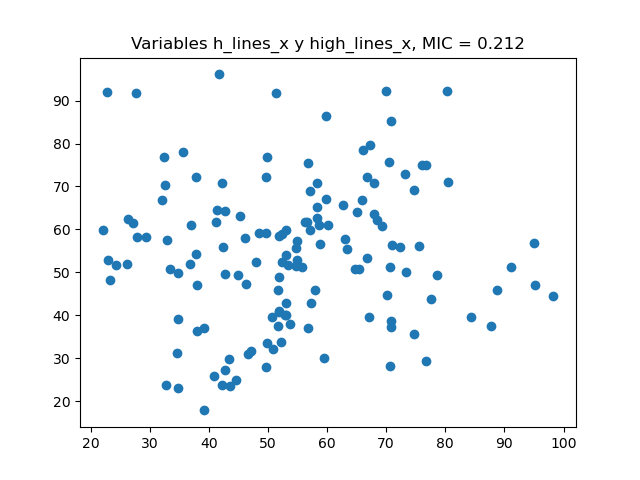
\includegraphics[scale=0.6]{h_lines_x_high_lines_x_.png}
		\caption{ MIC = 0.212}
		\end{figure}

		
\section[]{Correlaci\'on local} 

	%chen2010.pdf

	\subsection{Discucion sobre el coef.}

	donde se publico, como su ocupa, despcion en palabras

	La correlaci\'on local, tamb\'ien conodica como coeficiente no param\'etrico de Chen, o coeficiente de Chen. Este, sin realizar supuestos sobre distribuciones, detecta relaciones no lineales al invenstigar un mont\'on de correalciones locales. 

	\subsection{Definiciones}

	La definici\'on del m\'etodo est\'a basada en en el concepto de integrales de correlaci\'on, las cuales se definen de la siguiente forma:
	\begin{defn}
		$$
		I(r)=\lim _{N \rightarrow \infty}\left\{\frac{1}{N^{2}} \sum_{i, j=1}^{N} I\left(\left|z_{i}-z_{j}\right|<r\right)\right\}
		$$
	\end{defn}
	La integral de correlaci\'on cuantifica el el n\'umero promedio de vecinos dentro de un radio $r$. Notemos que esta definici\'on sigue teniendo sentido cuando los datos no son series de tiempo.

	Para desarrollar una medida de asociaci\'on entre vectores, $x$ e $y$, modificamos la definici\'on de $I(r)$ como sigue. Sean $z_i=(x_i,y_i)$ con $i=1,\dots, N$ las observaciones en el conjunto de datos. Sea $|z_i-z_j|$ la distancia euclidiana. Definimos $\hat{I}(r)=\frac{1}{N^{2}} \sum_{i, j=1}^{N} I\left(\left|z_{i}-z_{j}\right|<r\right)$. Las distancias obsevadas son adem\'as linealmente transformadas para que se encuentren entres 0 y 1 antes de calcular $\hat{I}$. Notemos que $\hat{I}$a tiene las propiedades de una funci\'on de distribuci\'on acumulativa. Es no decreciente entre 0 y 1 y continua por la derecha. La funci\'on $\hat{I}(r)$ descrive el patr\'on global de distancias entre vecinos. 

	Nuestro inter\'es principal es la definici\'on  de una metrica para cuantificar la asosiaci\'on no lineal estudiando patrones locale. Dado esto, definimos la densidad de vecinos $D$ de forma similar a la derivada de $\hat{I}$: 

	$$
		\hat{D}(r)= \frac{\vartriangle\hat{I}(r)}{\vartriangle r}
	$$

	Donde $\vartriangle\hat{I}(r)$ denota un cambio en $\hat{I}(r)$. La densidad de vecinos es evaluada en radio distreto r, con $r=0,1/m, 2/m, \dots, 1$  y $m$ es un grosor de malla arbitrario. Una funci\'on de suavizado autom\'atico usando validaci\'on cruzada es usada para elegir un \'optimo el tama\~no $m$ (Vilela et al. 2007) y se aplica para suavizar $D(r)$. En el paper, el tama\~no predeterminado $m$ se establece como $N$, el n\'umero de observaciones y en este trabajo usaremos el mismo $m$. El estad\'istico $\hat{D}$ es una aproximaci\'on discreta de $d\hat{I}(r)/d r$, la cual tiene las propiedades formales de una probabilidad funci\'on de densidad. Por lo tanto, con un ligero abuso de terminolog\'ia nos referimos a $\widehat{D}(r)$ como una distribuci\'on.

	En base a esto definimos la correlaci\'on local. Intuitivamente, las distancias entre los puntos de datos entre dos variables correlacionadas diferir\'ian de las distancias entre dos variables no correlacionadas. Sea $\widehat{D_0}(r)$ la estimaci\'on de una distribuci\'on nula, que se compone de dos vectores sin asociaci\'on. Definimos la correlaci\'on local ($\ell(r)$) como la desviaci\'on de D de la de la distribuci\'on nula a una distancia vecina dada r:

	$$
		\ell(r)=\widehat{D}(r)-\widehat{D}_{0}(r)
	$$

	Este enfoque no asume ninguna distribuci\'on param\'etrica. La flexibilidad de este m\'etodo facilita el cambio de la distribuci\'on nula a cualquier distribuci\'on de inter\'es. 
	
	Por ultimo, definimos el coficiente como de correlaci\'on local m\'axima, o coeficiente de Chen como:
	$$
		M=\max _{r}\{|\ell(r)|\}
	$$
	La interpretaci\'on de $\ell(r)$ como la diferencia de dos distribuciones implica que $M$ puede interpretarse como la distancia bajo la norma del supremo entre $\widehat{D}$ y $\widehat{D_0}$. En otras palabras, definimos el estad\'istico M como la desviaci\'on m\'axima entre dos densidades vecinas subyacentes.


\section[]{Correlaci\'on de Pearson}

	\subsection{Discucion sobre el coef.}
	
		donde se publico, como su ocupa, despcion en palabras
	 
	\section{Definiciones}
	
	El coef. se define como:
	\begin{equation}\label{pearson_orig}
		\rho_{X,Y}=\frac{cov(X,Y)}{\sigma_X\sigma_Y}
	\end{equation}
	
	Para una muestra de tama\~no $N$, tenemos:
	
	\begin{equation}\label{pearson_r}
		r=\frac{\sum_{i}^N\left(x_{i}-\bar{x}\right)\left(y_{i}-\bar{y}\right)}{\sqrt{\sum_{i}^n\left(x_{i}-\bar{x}\right)^{2}} \sqrt{\sum_{i}^n\left(y_{i}-\bar{y}\right)^{2}}}
	\end{equation}
	
	Con $x_i,y_i$ elementos de la muestra y $\bar{x},\bar{y}$ sus respectivos promedios.
	
	Hablar de The Ineffectiveness of the Correlation Coefficient for Image Comparisons
	
	\newpage